\documentclass[aspectratio=43]{beamer}

\usepackage[T1]{fontenc}
\usepackage[utf8]{inputenc}
\usepackage[english]{babel}
\usepackage{lmodern}
\usepackage{booktabs}
\usepackage{multirow}
\usepackage{subcaption}

%import the theme and packages for the code blocks
\input{code_blocks_theme.tex}

% Use Unipd as theme, with options:
% - pageofpages: define the separation symbol of the footer page of pages (e.g.: of, di, /, default: of)
% - logo: position another logo near the Unipd logo in the title page (e.g. department logo), passing the second logo path as option 
% Use the environment lastframe to add the endframe text
\usetheme[pageofpages=of]{Unipd}

\title{Charm hadrons reconstruction in ALICE\\}
\subtitle{}
\author[]{Pieripolli Leonardo, Pirazzo Tommaso, Ponchio Mattia, Secco Benedetto}

\date{10th February 2026}


\begin{document}
	\frame{\titlepage}
	\section{Logistic Regression on German Credit Data}
	\begin{frame}
		\begin{center}
			{\Huge \textbf{Logistic Regression on German Credit Data}}
		\end{center}
	\end{frame}
	\begin{frame}{The Dataset}
		\begin{enumerate}
			\item Original dataset contains both numerical (e.g. Age, credit amount, ...) and categorical data (e.g. Sex, Civil status, ...) $\rightarrow$ we used the numerical version provided by Strathclyde University.
			\item 1000 individuals with 24 features and a classifier for "good" (+1) and "bad" (-1) creditors.
		\end{enumerate}
		\begin{center}
			\textbf{Our goal:} sample from the target distribution of the posterior. 
		\end{center}
	\end{frame}
	
	\begin{frame}{The Model}
		\begin{center}
			\textbf{Bayesian Logistic Regression model.}
		\end{center}
		
		The target distribution is $p(\alpha, \beta \mid X, y) \propto p(y|X, \alpha, \beta) \, p(\alpha) \, p(\beta)$
		\begin{equation*}
			\propto \exp\left(
			-\sum_{i}\log\!\left(1+\exp\!\left\{-y_i\left(\alpha + x_i \cdot \beta\right)\right\}\right)
			-\frac{\alpha^2}{2\sigma^2}
			-\frac{1}{2\sigma^2}\,\beta \cdot \beta
			\right)
		\end{equation*}
		
		where:
		\begin{itemize}
			\item $x_i$ is a 24-dimensional vector of numerical predictors associated with a customer $i$.
			\item $y_i$ is $+1$ if the customer should receive credit, $-1$ otherwise.
			\item $\alpha$ is a scalar intercept term.
			\item $\beta$ is a vector of 24 regression coefficients.
			\item All predictors are normalized to have zero mean and unit variance.
			\item $\alpha$ and each element of $\beta$ are given given weak zero-mean normal priors with a \textbf{fixed} variance $\sigma^2 = 100$.
			
		\end{itemize}
		
	\end{frame}
	
	\begin{frame}{The Model: Likelihood}
		We assume that the probability of a customer being "good" depends on a linear combination of the features: 
		\begin{gather*}
			\eta_i = \alpha + x_i \beta \\
			p(y_i = 1 \mid x_i, \alpha, \beta) = \sigma(\eta_i)
		\end{gather*}
		where $\sigma(\eta_i) = \frac{1}{1 + e^{-\eta_i}}$ is the sigmoid logistic function.
		
		Therefore, because $y = \{-1, +1\}$
		$$
		\begin{cases}
			p(y_i = 1 | x_i) = \sigma(\eta_i) \\
			p(y_i = -1 | x_i) = 1 - \sigma(\eta_i) = \frac{e^{-\eta_i}}{1+e^{-\eta_i}} = \frac{1}{1 + e^{+\eta_i}}\\
		\end{cases}
		$$
		
		And we obtain the compact form:
		\begin{equation*}
			p(y_i | x_i) = \sigma(y_i \eta_i) = \frac{1}{1 + e^{-y_i \eta_i}}
		\end{equation*}
	\end{frame}
	
	\begin{frame}{Realized average acceptance probability h}
		\begin{figure}
			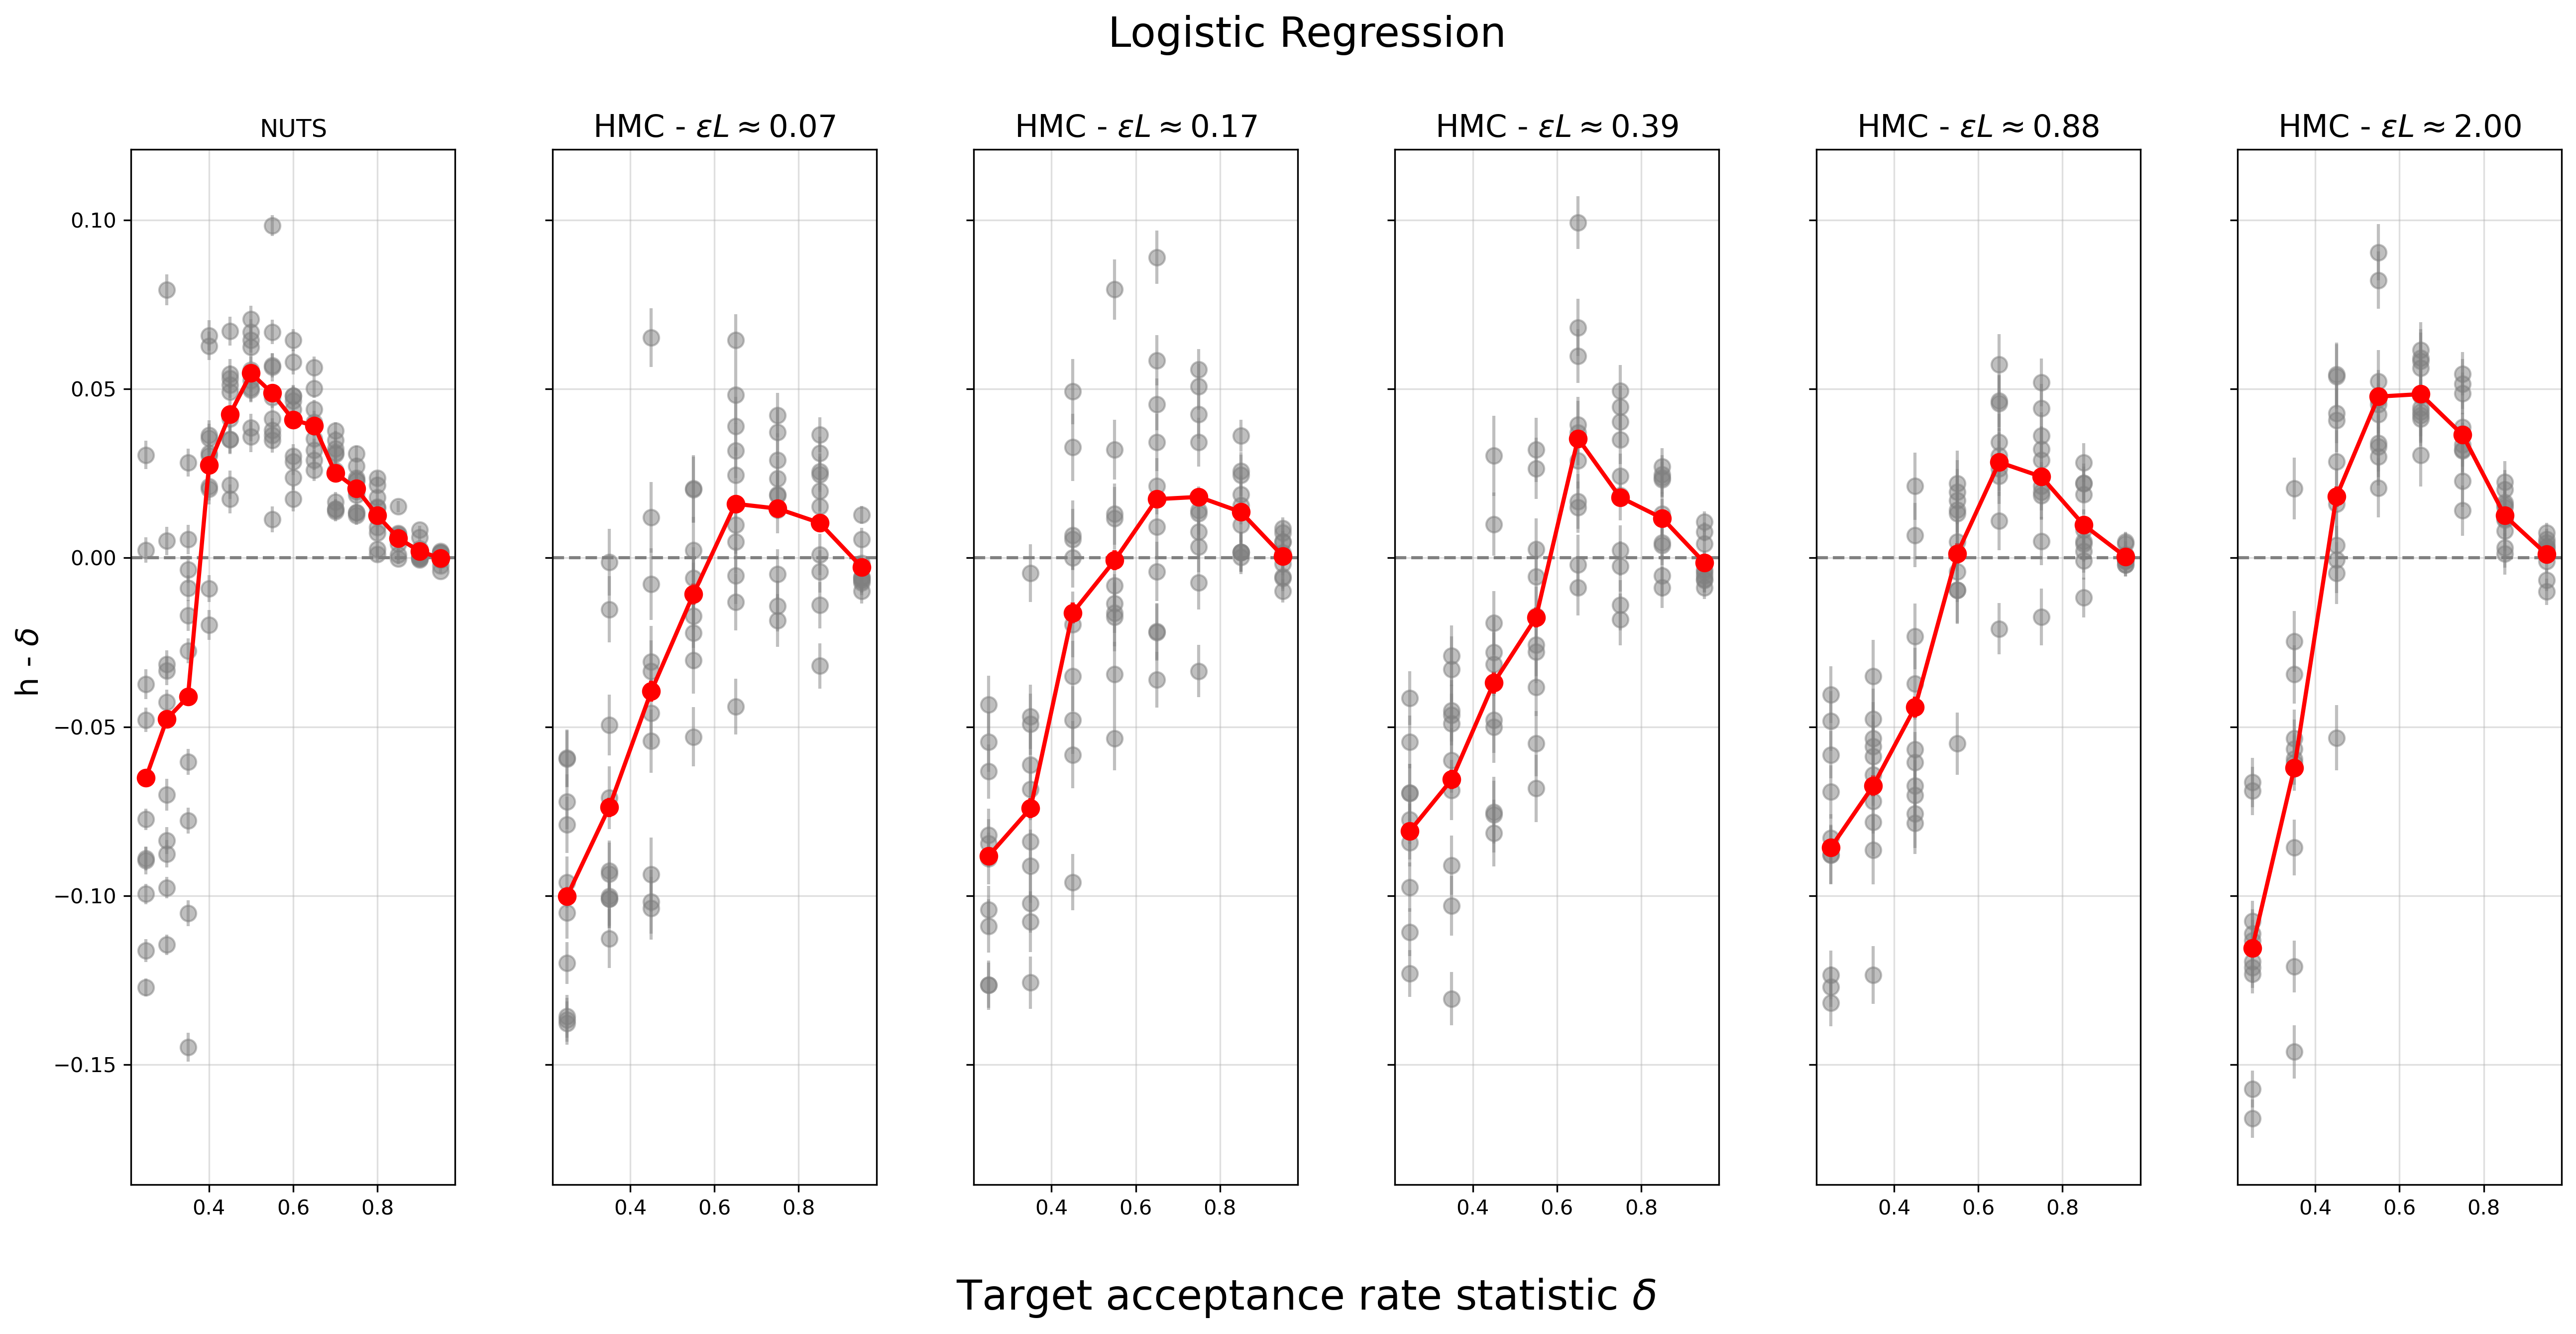
\includegraphics[width=1.0\textwidth]{images/Combined_LR_h-delta.png}
			\caption{Each gray point is obtained by averaging across all 4 chains. The computation has been repeated 10 times for each value of $\delta$. In red the average across all repetitions.}
		\end{figure}
	\end{frame}
	
		\begin{frame}{Acceptance probability comparison with paper}
		\begin{figure}[ht]
			\centering
			
			\begin{subfigure}[b]{0.90\textwidth}
				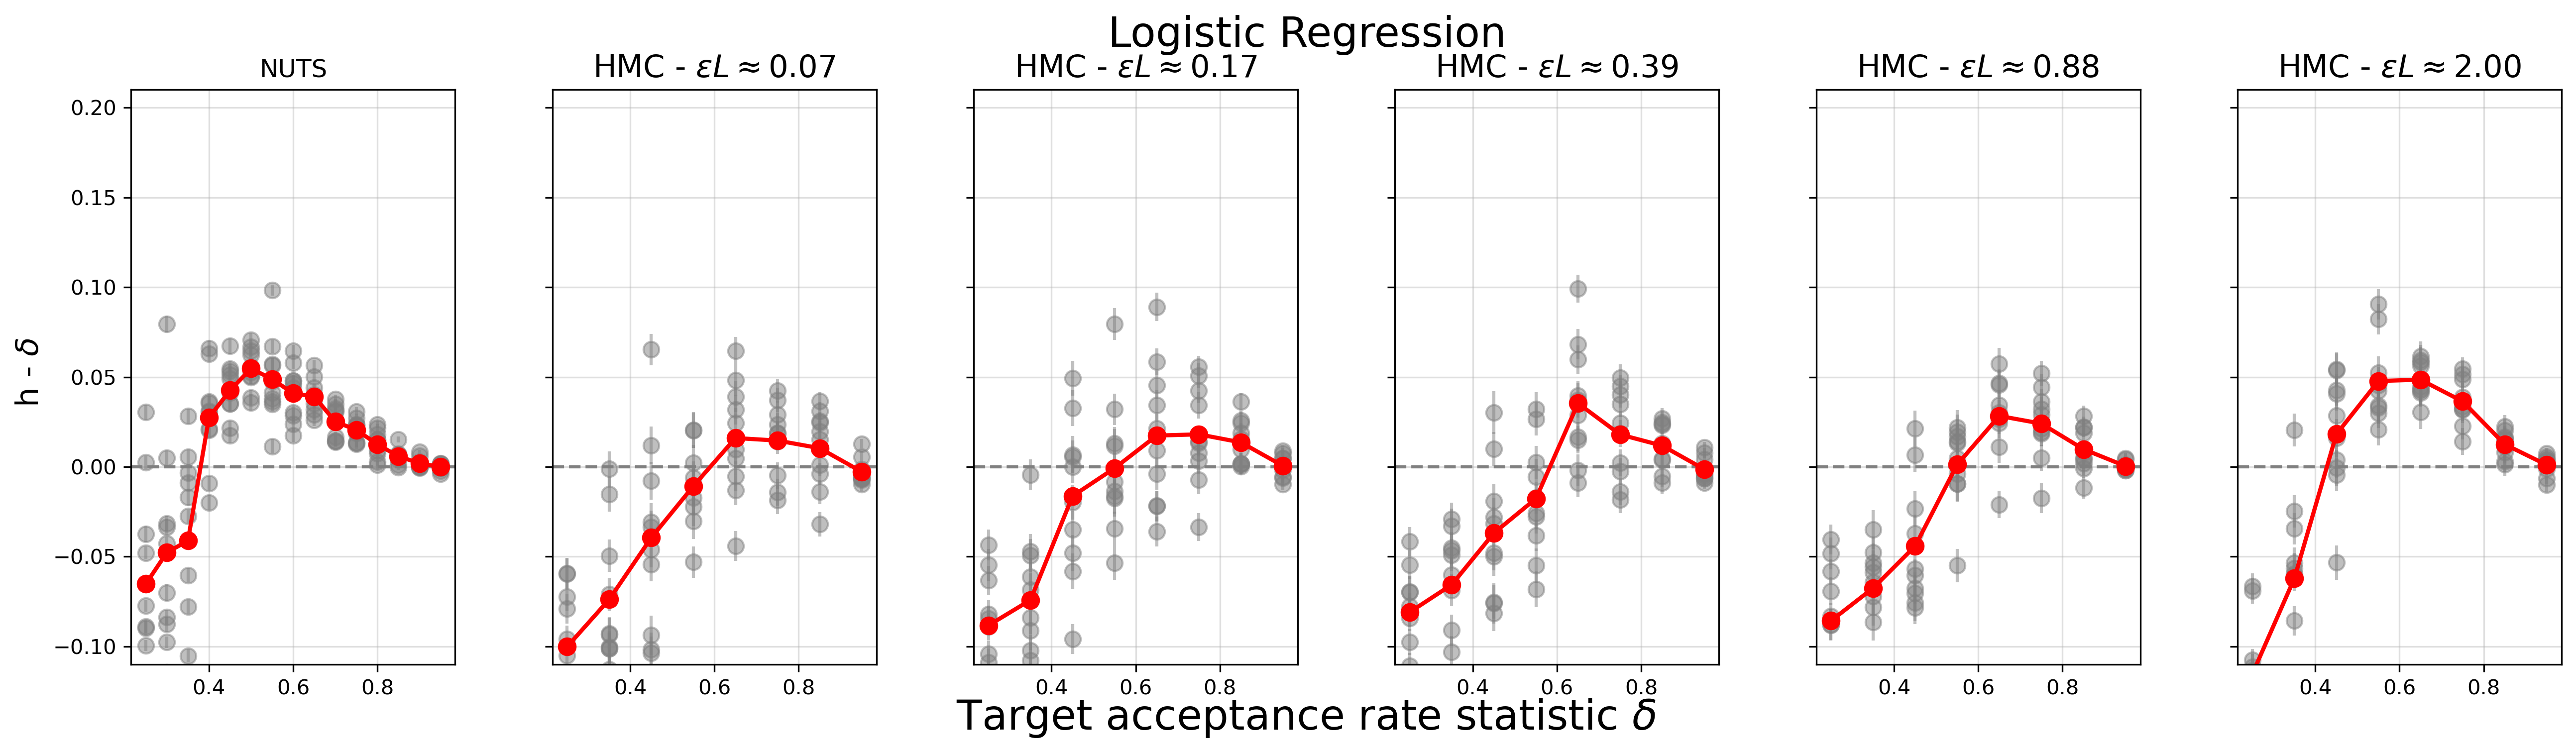
\includegraphics[width=1\linewidth]{images/Combined_LR_h-delta_paper-like.png}
				\label{fig:Ng1}
				\caption{\tiny Our results}
			\end{subfigure}
			
			\begin{subfigure}[b]{0.90\textwidth}
				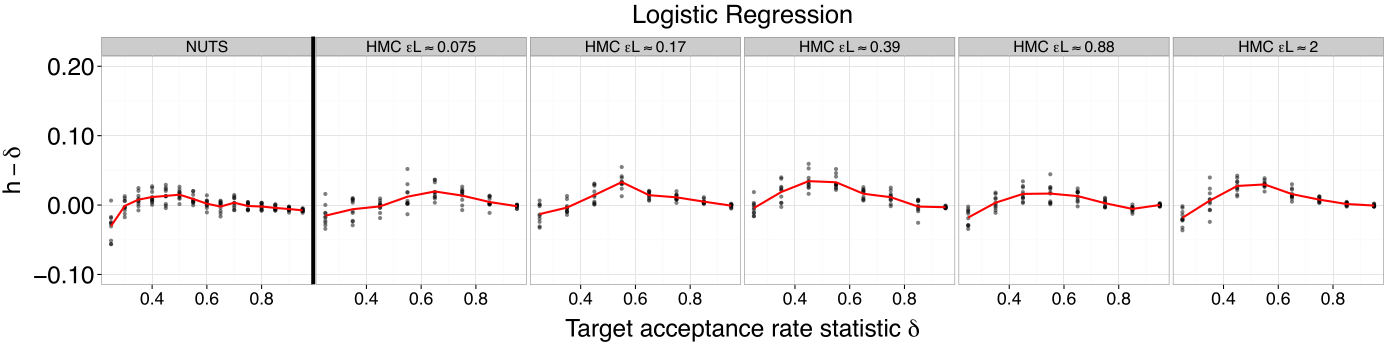
\includegraphics[width=1\linewidth]{images/paper_LR-h-delta.png}
				\caption{\tiny Paper's results.}
				\label{fig:Ng2}
			\end{subfigure}
			
		\end{figure}
	\end{frame}
	
	\begin{frame}{ESS efficiency}
		\begin{figure}
			\includegraphics[width=1.0\textwidth]{images/Combined_LR_ESS-per-grad.png}
			\caption{Each gray point is obtained by taking the minimum ESS per gradient across all 4 chains for all variables, considering both mean and variance. In red the average across all repetitions.}
		\end{figure}
	\end{frame}
	
	\begin{frame}{ESS efficiency comparison with paper}
		\begin{figure}[ht]
			\centering
			
			\begin{subfigure}[b]{0.90\textwidth}
				\includegraphics[width=1\linewidth]{images/Combined_LR_ESS-per-grad_paper-like.png}
				\label{fig:Ng1}
				\caption{\tiny Our results}
			\end{subfigure}
			
			\begin{subfigure}[b]{0.90\textwidth}
				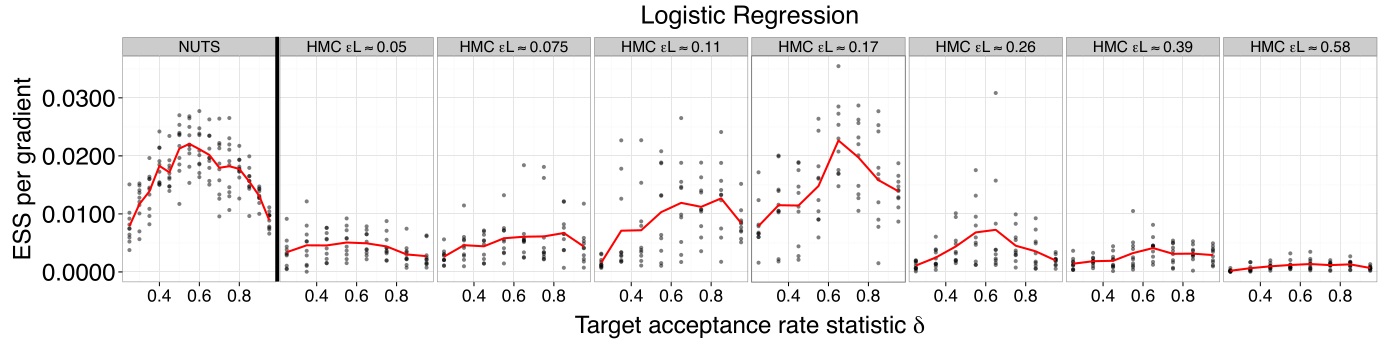
\includegraphics[width=1\linewidth]{images/paper_LR-ESS-per-grad.png}
				\caption{\tiny Paper's results.}
				\label{fig:Ng2}
			\end{subfigure}
			
		\end{figure}
	\end{frame}
	
	\section{Hierarchical Logistic Regression on German Credit Data}
	\begin{frame}
	\begin{center}
		{\Huge \textbf{Hierarchical Logistic Regression on German Credit Data}}
	\end{center}
	\end{frame}
	\begin{frame}{Changes from previous model}
		\begin{enumerate}
			\item We expand the predictor vectors by including two-way interactions ($x_i \cdot x_j$, $i \neq j$), resulting in $\binom{24}{2} = 276 + 24 =$ 300-dimensional vectors of predictors \textbf{x} and a 300-dimensional vector of coefficients \textbf{$\beta$}.
			\item The variance parameter in
			the prior on $\alpha$ and $\beta$ is given an exponential prior and estimated as well.
			\item  We set $\lambda = 0.01$, yielding a weak exponential prior distribution on $\sigma^2$,  whose mean and standard deviation are 100.
		\end{enumerate}
		
		\begin{center}
			$\Downarrow$
			
			These changes make for a more challenging problem: the posterior is in higher dimensions and the variance term $\sigma^2$ interacts strongly with the remaining 301 variables.
		\end{center}
	\end{frame}
	
	\begin{frame}{The paper's posterior}
		$p(\alpha, \beta , \sigma^2 \mid X, y) \propto  p(y|X, \alpha, \beta) \, p(\beta| \sigma^2) p(\alpha|\sigma^2) p(\sigma^2) \, \propto
		$
		$$
		\exp\left(
		-\sum_{i}\log\!\left(1+\exp\!\left\{-y_i x_i \cdot \beta\right\}\right)
		-\frac{\alpha^2}{2\sigma^2}
		-\frac{1}{2\sigma^2}\,\beta \cdot \beta - \frac{N}{2}\log{\sigma^2} - \lambda \sigma^2
		\right)
		$$
		where N = 1000 is the number of customers.
		
		\begin{center}
			{\Large \textbf{However...}}
			
			\Large
			that should instead be $\mathbf{\frac{D+1}{2}}$ where D is the dimension of $\beta$ (300).
			
		\end{center}
		
		\begin{center}
			(Also the intercept term $\alpha$ is missing in the (log)-likelihood)
		\end{center}
	\end{frame}

	\begin{frame}{Motivation}
		Now the variance $\sigma^2$ on $\alpha$ and $\beta$ is inferred from data, therefore in the log-posterior for these parameters we get:
		\begin{align*}
			\log p(\alpha \mid \sigma^2) &= -\frac{1}{2}\log\left(2\pi\sigma^2\right) - \frac{\alpha^2}{2\sigma^2} \\
			\log p(\beta \mid \sigma^2) &= -\frac{D}{2}\log\left(2\pi\sigma^2\right) - \frac{\beta^T \beta}{2\sigma^2}
		\end{align*}
		
		So their total contribution to the log-posterior is:
		\begin{equation*}
			-\frac{\alpha^2 + \beta^T \cdot \beta}{2\sigma^2} -\frac{D+1}{2}\log(\sigma^2)
		\end{equation*}
		
		Therefore, the log-posterior we sampled from is proportional to:
		\begin{equation*}
		-\sum_{i}\log\!\left(1+\exp\!\left\{-y_i\left(\alpha + x_i \cdot \beta\right)\right\}\right)
			-\frac{\alpha^2}{2\sigma^2}
			-\frac{\beta^T\beta}{2\sigma^2}\, - \frac{D+1}{2}\log{\sigma^2} - \lambda \sigma^2
		\end{equation*}
		
	\end{frame}
	
	\begin{frame}{Realized average acceptance probability h}
		\begin{figure}
			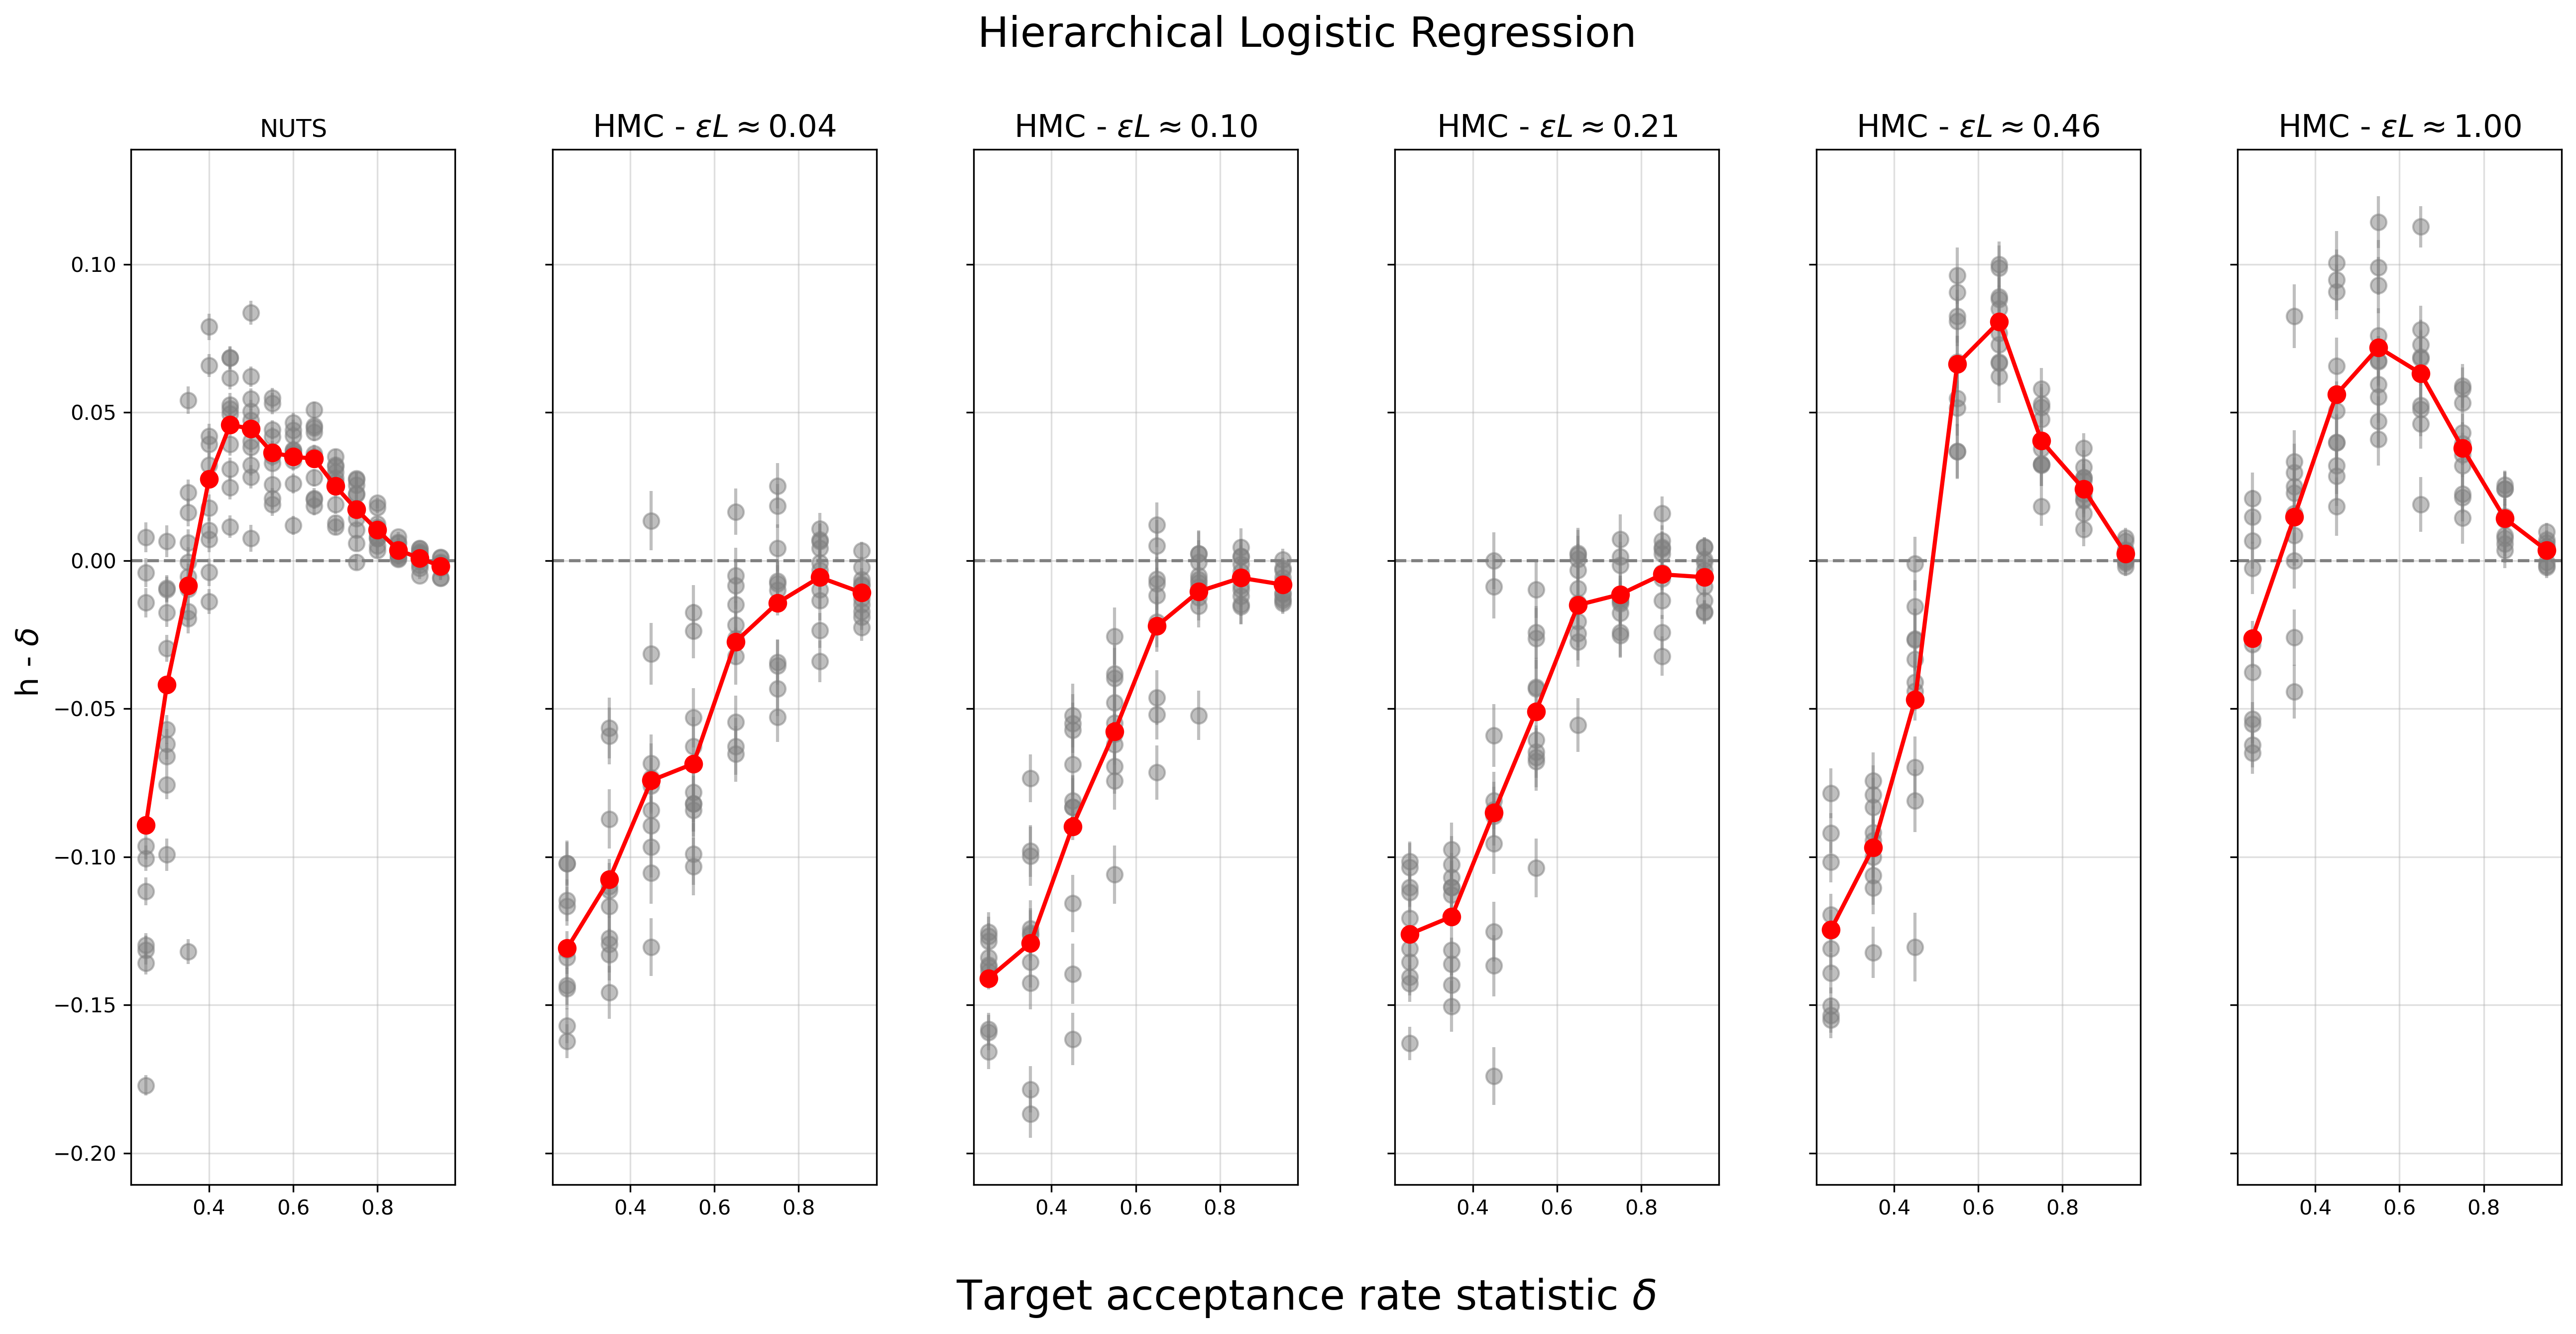
\includegraphics[width=1.0\textwidth]{images/Combined_HLR_h-delta.png}
		\end{figure}
	\end{frame}
	
	\begin{frame}{ESS efficiency}
		\begin{figure}
			\includegraphics[width=1.0\textwidth]{images/Combined_HLR_ESS-per-grad.png}
		\end{figure}
	\end{frame}
	
		\begin{frame}{ESS efficiency: HMC example}
		\begin{figure}
			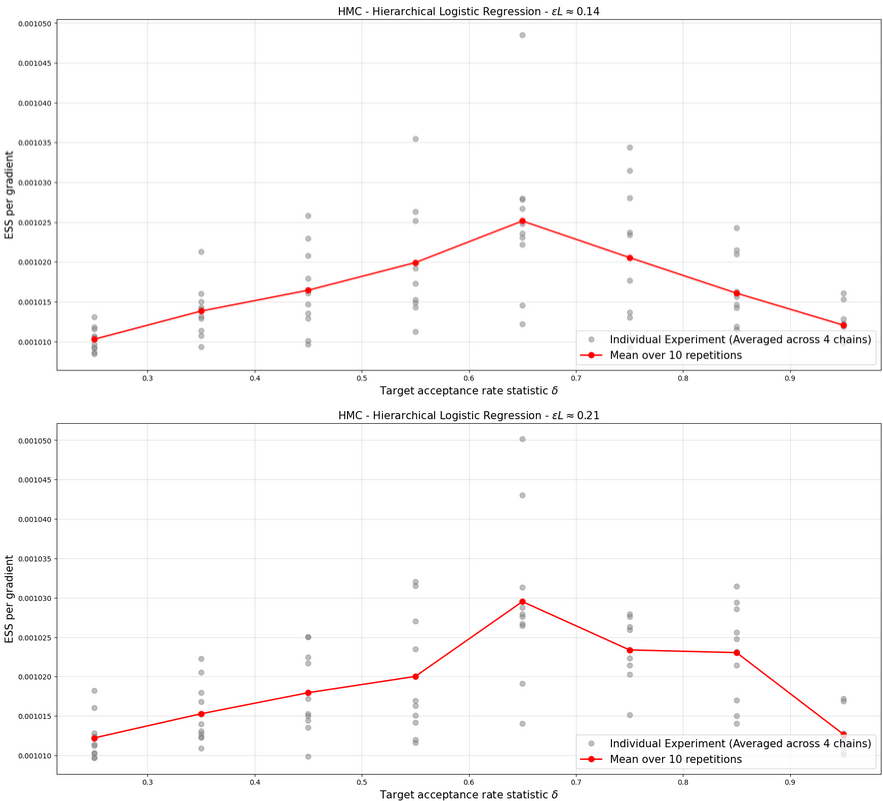
\includegraphics[width=0.80\textwidth]{images/example.png}
		\end{figure}
	\end{frame}
	
	\begin{frame}{NUTS Tree Depth Histogram}
		\begin{figure}
			\centering
			\begin{subfigure}{.53\textwidth}
				\centering
				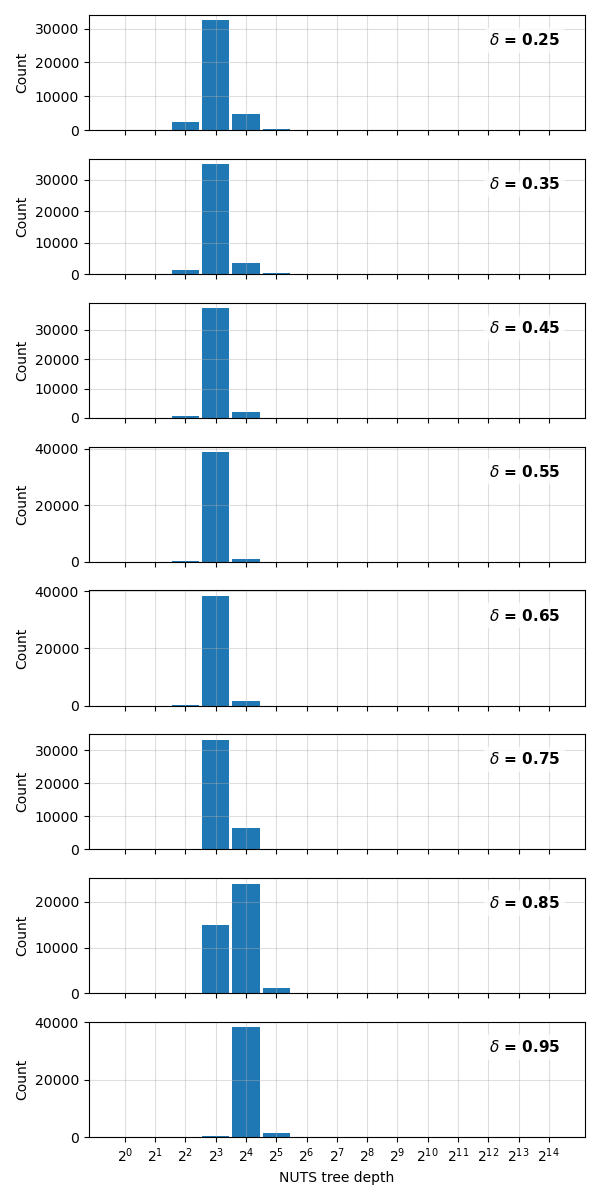
\includegraphics[width=.6\linewidth]{images/LR_NUTS_Counts.png}
				\caption{Logistic Regression Tree Depths.}
				\label{fig:sub1}
			\end{subfigure}%
			\begin{subfigure}{.53\textwidth}
				\centering
				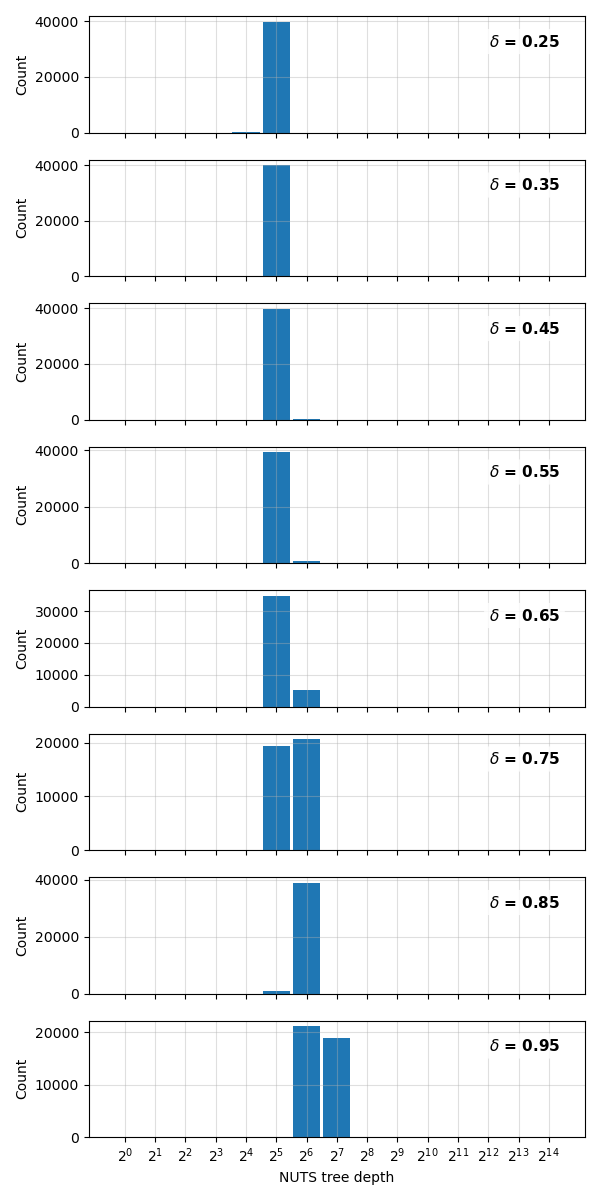
\includegraphics[width=.6\linewidth]{images/HLR_NUTS_Counts.png}
				\caption{Hierarchical LR Tree Depths.}
				\label{fig:sub2}
			\end{subfigure}
			\label{fig:counts}
		\end{figure}
	\end{frame}
	
\end{document}